% !TeX document-id = {5c05c331-134f-48f1-8db3-fd32c67a647b}
%%%%%%%%%%%%%%%%%%%%%%%%%%%%%%%%%%%%%%%%%
% Journal Article
% LaTeX Template
% Version 2.0 (February 7, 2023)
%
% This template originates from:
% https://www.LaTeXTemplates.com
%
% Author:
% Vel (vel@latextemplates.com)
%
% License:
% CC BY-NC-SA 4.0 (https://creativecommons.org/licenses/by-nc-sa/4.0/)
%
% NOTE: The bibliography needs to be compiled using the biber engine.
%
%%%%%%%%%%%%%%%%%%%%%%%%%%%%%%%%%%%%%%%%%

% Magic comments for TeXStudio
% !TeX program = pdflatex
% !BIB program = biber
% !TeX encoding = utf8
% !TeX spellcheck = en_US

%----------------------------------------------------------------------------------------
%	PACKAGES AND OTHER DOCUMENT CONFIGURATIONS
%----------------------------------------------------------------------------------------

\documentclass[
	a4paper, % Paper size, use either a4paper or letterpaper
	10pt, % Default font size, can also use 11pt or 12pt, although this is not recommended
	unnumberedsections, % Comment to enable section numbering
	twoside, % Two side traditional mode where headers and footers change between odd and even pages, comment this option to make them fixed
	onecolumn,
]{LTJournalArticle}

\bibliography{sample.bib} % BibLaTeX bibliography file

\runninghead{Shortened Running Article Title} % A shortened article title to appear in the running head, leave this command empty for no running head

\footertext{\textit{} (2024) 12:533-684} % Text to appear in the footer, leave this command empty for no footer text

\setcounter{page}{1} % The page number of the first page, set this to a higher number if the article is to be part of an issue or larger work

% Main header file
% % % % % % % % % % % % % % % % % % % % % % % % % % % % % % % % % % % % % % % % %
%
% OSTReport -- Additional packages frequently used in reports
%
% % % % % % % % % % % % % % % % % % % % % % % % % % % % % % % % % % % % % % % % %

% Mathematical equations
\usepackage{amsmath}
\usepackage{amssymb}
\usepackage{bm}
\usepackage{MnSymbol}
%\usepackage{breqn}

% Tables
\usepackage{multirow}
\usepackage{tabularx}
\usepackage{booktabs}

% Figures
\usepackage{pdfpages}
\usepackage{epstopdf}
%\usepackage[outdir=./]{epstopdf}

% Quotation marks
\usepackage{csquotes}
\setquotestyle[quotes]{german}

% Si Units
\usepackage{siunitx}
\sisetup{detect-all,sticky-per,per-mode=symbol}

% Multicolumn documents and sections
\usepackage{multicol}

\PassOptionsToPackage{svgnames,x11names,dvipsnames}{xcolor}
\usepackage[most]{tcolorbox}

%----------------------------------------------------------------------------------------
%	TITLE SECTION
%----------------------------------------------------------------------------------------

\title{Introduction for Mac Users} % Article title, use manual lines breaks (\\) to beautify the layout

% Authors are listed in a comma-separated list with superscript numbers indicating affiliations
% \thanks{} is used for any text that should be placed in a footnote on the first page, such as the corresponding author's email, journal acceptance dates, a copyright/license notice, keywords, etc
\author{%
	Nathan Hoffman\textsuperscript{1}
}

% Affiliations are output in the \date{} command
\date{\footnotesize\textsuperscript{\textbf{1}}University of Bern}

% Full-width abstract
\renewcommand{\maketitlehookd}{%
	\begin{abstract}
		\noindent This is a short introduction for mac users on how to install the \LaTeX-distribution \textbf{mactex} and the \LaTeX-editor \textbf{TexStudio} via \textbf{Homebrew}.
	\end{abstract}
}

%----------------------------------------------------------------------------------------

\begin{document}

\maketitle % Output the title section

%----------------------------------------------------------------------------------------
%	ARTICLE CONTENTS
%----------------------------------------------------------------------------------------

\section{Requirements}
Before we can start with writing a documents some programs have to be installed. In order to do so a package manger like \emph{Homebrew} can be used. 
In order to install Homebrew, open up your terminal (cmd + spacebar, and type in terminal) and paste this code into it:
\begin{verbatim}
	/bin/bash -c "$(curl -fsSL https://raw.githubusercontent.com/Homebrew/install/HEAD/install.sh)"
\end{verbatim}

After the download has completed, follow the instructions which are presented in the terminal. There are two commands which have to run and after that \emph{Homebrew} should work.

\section{Packages}
The following packages will be needed:
\begin{itemize}
	\item MacTex
	\item TexStudio
	\item Git (if XCode is installed already, then Git should be installed as well.)
\end{itemize}

The following command must be pasted into the terminal, so that MacTex is installed:
\begin{verbatim}
	brew install --cask mactex
\end{verbatim}

After MacTex has been installed, the \LaTeX-editor TexStudio can be installed with:
\begin{verbatim}
	brew install --cask texstudio
\end{verbatim}

If Git is not installed yet, then you can run the command:
\begin{verbatim}
	brew install git
\end{verbatim}

Now, all required packages are installed.

\section{Git basics}
In order to use git, first create a GitHub account. You can sign up at \href{https://github.com}{\textcolor{red}{Github}}.
\subsection{git clone}
The first command which you will need is \emph{git clone}. With \emph{git clone} you can clone a repository. A repository is where all the code will be kept and where the updates will be added to. 

So that you can clone a repository, search for green \emph{\textcolor{green}{Code}} button and click on to the SSH tab and copy the link which you see. These links usually start with \textbf{git@github.com}...
\begin{figure}[h!]
	\centering
	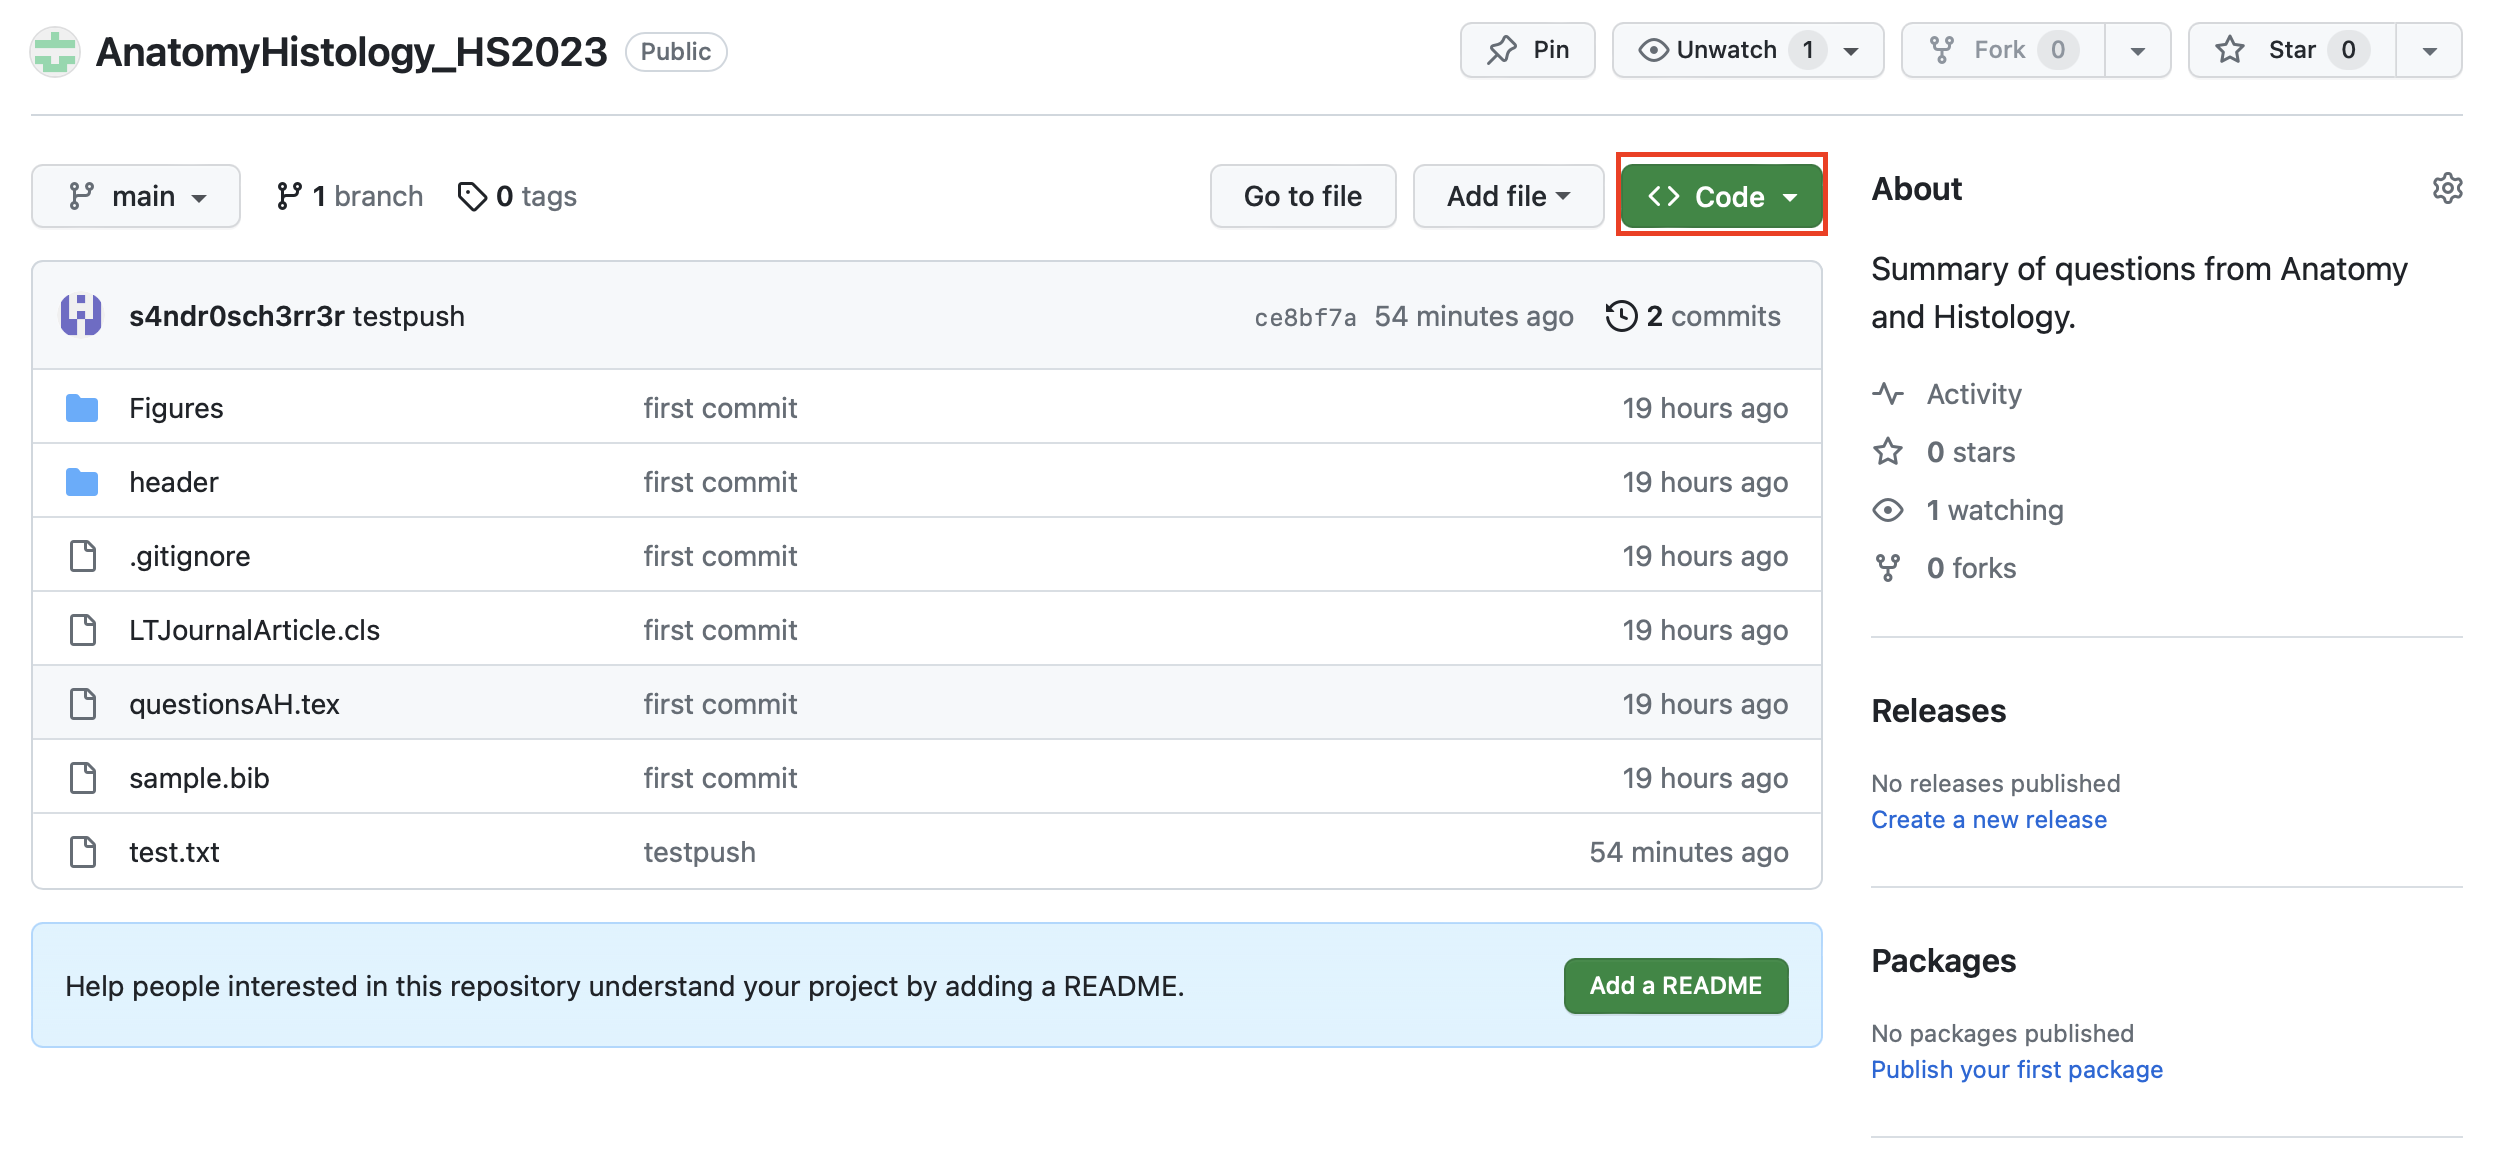
\includegraphics[width=0.5\linewidth]{codebtn.png}
\end{figure}

After you have copied the link, create a folder in which the repository should be cloned into. 
In the terminal open this path of the folder and write the command or any other repository which you want to clone:
\begin{verbatim}
	git clone git@github.com:BME-Students/AnatomyHistology_HS2023.git
\end{verbatim}

After you have cloned the repository, you can make changes to the files. They, however, are not affected in the main repository. In order to add these changes to the repository you first have to use the command \emph{git add} which will be described in the next section.

\subsection{git add}
In order to make changes to the repository on GitHub, you can add the files or also an individual file with the \emph{git add} command. With this command you prepare a file to be commited to the repository. 

With the command 
\begin{verbatim}
	git add \emph{filename.tex}
\end{verbatim}
you can add a single file for commiting and with
\begin{verbatim}
	git add .
\end{verbatim}
you add all files which have been changed.

\subsection{git commit}
With the following command
\begin{verbatim}
	git commit -m "add your comment"
\end{verbatim}
you commit the files. This means that the following changes will be pushed to the repository. 
With the \emph{-m} you leave a comment in after the \emph{"comment"}. Every commit also has a comment with a short description, what has been changed, e.g. "make changes to filename.tex" or "add images for documentation".

\subsection{git push}
With \emph{git push}  the changes are finally pushed to the repository and other people can now see your changes.
%----------------------------------------------------------------------------------------
%	 REFERENCES
%----------------------------------------------------------------------------------------

% \printbibliography % Output the bibliography

%----------------------------------------------------------------------------------------

\end{document}
